% !TEX TS-program = xelatex
% !TEX encoding = UTF-8 Unicode
% !Mode:: "TeX:UTF-8"
%\documentclass[bachelor,nocolorlinks, printoneside]{seuthesis} % 本科
% \documentclass[master]{seuthesis} % 硕士
% \documentclass[doctor]{seuthesis} % 博士
\documentclass[engineering]{seuthesis} % 工程硕士
\usepackage{CJK,CJKnumb}
\usepackage{amsmath}
\usepackage{amsfonts} 
\usepackage{bm} 
\usepackage{algorithm}
\usepackage{algorithmicx}
\usepackage{algpseudocode}
\usepackage{subfigure}

\floatname{algorithm}{算法}
\renewcommand{\algorithmicrequire}{\textbf{输入:}}
\renewcommand{\algorithmicensure}{\textbf{输出:}}
 % 这里是导言区

\begin{document}
\categorynumber{000} % 分类采用《中国图书资料分类法》
\UDC{000}            %《国际十进分类法UDC》的类号
\secretlevel{公开}    %学位论文密级分为"公开"、"内部"、"秘密"和"机密"四种
\studentid{163521}   %学号要完整,前面的零不能省略。

\title{基于XXX的YYY的设计与实现}{}{The Design and Implementation of Network Intrusion Detection System Based on the Long Short-Term Memory Technology}{}
\author{丁亚雷}{Yalei Ding}
\advisor{翟玉庆}{教授}{Yuqing Zhai}{Prof.}
\coadvisor{潘文彬}{}{Wenbing Pan}{} % 没有% 可以不填

\degree{工程硕士} % 详细学位名称
\major[12em]{计算机技术}
\submajor{计算机技术}
\defenddate{答辩日期}
\authorizedate{学位授予日期}
\department{计算机科学与工程}{department name}
\duration{2019年1月—2019年6月}
\address{}
%\thanks{本论文获国家XXX计划项目(2012AA00A00)和国家杰出青年科学基金项目(01234567)资助。}
\maketitle

\begin{abstract}{深度学习}
\seuabsstyle
摘要
\end{abstract}

\begin{englishabstract}{Deep Learning}
\seueabsstyle
Abstract
\end{englishabstract}

\tableofcontents


\begin{Main} % 开始正文

\chapter{绪论}
\section{研究背景}


\section{国内外研究现状}

\subsection{YYY}


\subsection{XXX}


\subsection{基于XXX的YYY}

\section{研究内容及意义}YYY

\section{组织结构}
\section{本章小结}


\chapter{相关技术的研究}

\section{测}


\section{深度学习}
有人的地方就有江湖,江湖险恶。


\section{本章小结}
本章小结

\chapter{分析}
\section{需求}。

\section{其他需求}


\section{xxx}


\section{本章小结}
本章主要介绍了的基本概念、原理。

\chapter{系统设计与实现}

\section{系统模型架构}

\subsection{a}
a

\subsection{b}
b

\subsection{c}


\subsection{d}


\section{本章小结}
本章介绍了心法和内功的关系。

\chapter{系统运行与测试}

\section{系统功能测试}

\subsection{a}
a

\subsection{b}
bbb

\subsection{c}
ccc
\subsection{d}
ddd

\section{测试结果与分析}


\section{本章小结}

\chapter{总结与展望}
\section{本文工作总结}
本文工作总结

\section{未来工作}

本章对全文工作进行了回顾和总结。

\section{数学公式}
\subsection{简单的数学公式}
\textbf{卷积}(\textbf{convolution})在图像分析的线性方法中是一种重要的运算。卷积是一个积分,反映一个函数$f(t)$在另一个函数上$h(t)$移动时所重叠的量。函数$f$和$h$在有限域$[0,t]$上的$1D$卷积$f*h$由下式给出:
 $$(f*h)(t) \equiv \int_0^t {f(\tau )h(t - \tau )d\tau } $$

\subsection{带自动编号的公式}
这里可以限定在$[0,t]$区间,原因是我们假设负坐标部分的值是0。为了准确起见,我们还可以将卷积积分的上限扩展为$( - \infty ,\infty )$:
\begin{equation}(f*h)(t) \equiv \int_{ - \infty }^\infty  {f(\tau )h(t - \tau )d\tau }  = \int_{ - \infty }^\infty  {f(t - \tau )h(\tau )d\tau }
  \end{equation} 

\subsection{带等号对齐的公式}
卷积可以推广到更高维。令$2D$函数$f$和$h$的卷积$g$记为$f*h$,则有:
\begin{equation}
\begin{aligned}
(f*h)(x,y) &= \int_{ - \infty }^\infty  {\int_{ - \infty }^\infty  {f(a,b)h(x - a,y - b)} } dadb\\
 &= \int_{ - \infty }^\infty  {\int_{ - \infty }^\infty  {f(x - a,y - b)h(a,b)} } dadb\\
\end{aligned}
\end{equation}

\section{伪代码}
在写论文的时候我们通常要写伪代码,伪代码里面有时甚至还要包含数学公式(如根号一类的)。伪代码会自动找一个比较好的位置插入图片。

\begin{algorithm}
    \caption{用归并排序求逆序数}
    \begin{algorithmic}[1] %每行显示行号
        \Require $Array$数组,$n$数组大小
        \Ensure 逆序数
        \Function {MergerSort}{$Array, left, right$}
            \State $result \gets 0$
            \If {$left < right$}
                \State $middle \gets (left + right) / 2$
                \State $result \gets result +$ \Call{MergerSort}{$Array, left, middle$}
                \State $result \gets result +$ \Call{MergerSort}{$Array, middle, right$}
                \State $result \gets result +$ \Call{Merger}{$Array,left,middle,right$}
            \EndIf
            \State \Return{$result$}
        \EndFunction
        \State
        \Function{Merger}{$Array, left, middle, right$}
            \State $i\gets left$
            \State $j\gets middle$
            \State $k\gets 0$
            \State $result \gets 0$
            \While{$i<middle$ \textbf{and} $j<right$}
                \If{$Array[i]<Array[j]$}
                    \State $B[k++]\gets Array[i++]$
                \Else
                    \State $B[k++] \gets Array[j++]$
                    \State $result \gets result + (middle - i)$
                \EndIf
            \EndWhile
            \While{$i<middle$}
                \State $B[k++] \gets Array[i++]$
            \EndWhile
            \While{$j<right$}
                \State $B[k++] \gets Array[j++]$
            \EndWhile
            \For{$i = 0 \to k-1$}
                \State $Array[left + i] \gets B[i]$
            \EndFor
            \State \Return{$result$}
        \EndFunction
    \end{algorithmic}
\end{algorithm}

\section{插入图片}
在使用该命令的时候,图片会自动找一个他觉得比较好的位置插入图片,我们就不需要担心前面改了文字之后后面的格式乱掉。
\begin{figure}[htbp!]
\centering 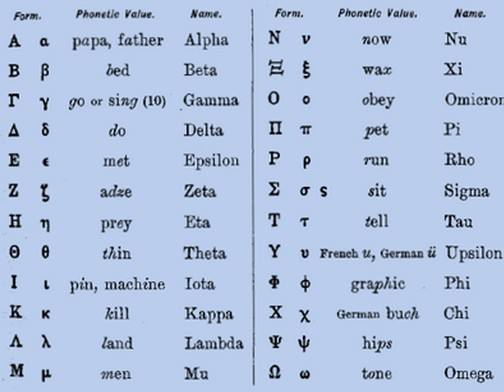
\includegraphics[width=0.9\textwidth]{img/test.jpg} \caption{图片的一个简单应用场景}
\end{figure}

\begin{figure}
\centering
\subfigure[the first subfigure]{
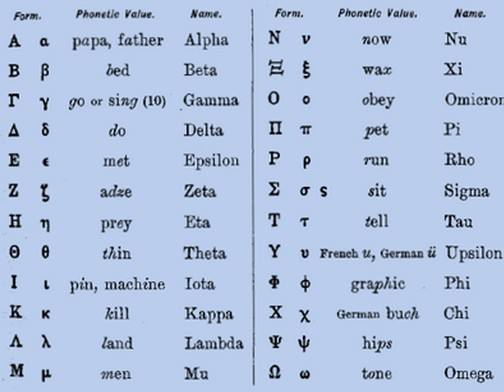
\includegraphics[width=0.4\textwidth]{img/test.jpg} 
}
\subfigure[the second subfigure]{
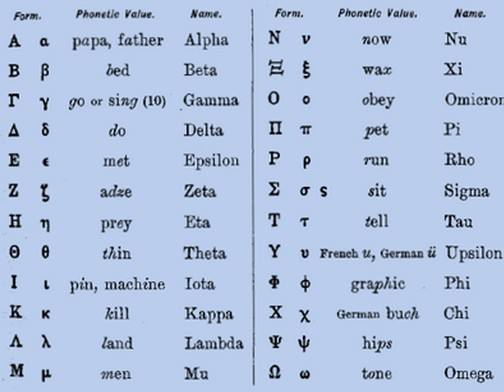
\includegraphics[width=0.4\textwidth]{img/test.jpg} 
}
\caption{子图应用场景}
\end{figure}

\section{引用论文}
使得论文符合要求\cite{Yao:2015ix}\cite{seucover}\cite{test1}\cite{test}\cite{R1}。

\end{Main} % 结束正文

\begin{Acknowledgement}{}
\seuackstyle
这次的毕业论文设计总结是在我的指导老师xxx老师亲切关怀和悉心指导下完成的。从毕业设计选题到设计完成,x老师给予了我耐心指导与细心关怀,有了莫老师耐心指导与细心关怀我才不会在设计的过程中迷失方向,失去前进动力。x老师有严肃的科学态度,严谨的治学精神和精益求精的工作作风,这些都是我所需要学习的,感谢x老师给予了我这样一个学习机会,谢谢!

  感谢与我并肩作战的舍友与同学们,感谢关心我支持我的朋友们,感谢学校领导、老师们,感谢你们给予我的帮助与关怀;感谢肇庆学院,特别感谢计算机科学与软件学院四年来为我提供的良好学习环境,谢谢!
\end{Acknowledgement}

% 参考文献
\bibliography{seuthesis}



\newpage
\printindex % 索引

%\begin{thebibliography}{99}


%\bibliographystyle{ieee}
%\bibliography{seuthesis}


\end{document}
